\chapter{Case Study: Comparing Conflict Among Forest Ecosystem Services Under Varying Sustainability Certifications}
\label{ch:caseStudyFSC}
This is where we describe why this chapter exists (demonstrate the conflict metrics on different frontiers).

\section{Introduction}
\label{sec:intro}
This is where we describe the problem.

\section{The multi-objective model}
This is where we describe the model.

\subsubsection{Notation}
We use the following notation in the development of the model:

\paragraph{Model parameters}
\begin{itemize}
\item \textbf{$i \in I$:} the set of forest stands comprising the Drink Area ($|I| = 303$)

\item \textbf{$a_i$:} the area of stand $i$

\item \textbf{$r \in R$:} the set of fuel removal prescriptions:
	$$
	r =
	\begin{cases}
	1 &\text{ fuel removals in the first period (2015-2035)}\\
	2 &\text{ fuel removals in the second period (2035-2055)}\\
	3 &\text{ fuel removals in both periods}\\
	0 &\text{ no fuel removals performed in either period}
	\end{cases}
	$$
	
\item \textbf{$F_{i,r}$:} the area-weighted fire hazard rating of stand $i$ at the end of the planning horizon if prescribed to fuel removal schedule $r$. For instance, if a stand $i$ under fuel removal schedule $r$ has a fire hazard rating of 4 in the year 2095, and its area is 10 hectares, then $F_{i,r} = 40$. The metric for fire hazard rating used in this analysis was developed by Schroder \textit{et al.} \cite{schroder2016multi} specifically for the Drink Area. It uses fire characteristics from the set of fuel models proposed by Anderson \cite{anderson1982aids} in order to assign a fire hazard rating. We expand the rating system to include fuel models not present in Schroder \textit{et al.} See Table \ref{tab:firehazards} for the mapping of fuel models to fire hazard ratings.

The USFS's Climate-Forest Vegetation Simulator (Climate-FVS) was used to generate the fuels and vegetation characteristics of the stands in order to determine their fire hazard rating. Initial vegetation data for Climate-FVS came from the 2012 GNN structure map (\url{http://lemma.forestry.oregonstate.edu/data/structure-maps}) from Oregon State University's Landscape Ecology, Modeling, Mapping \& Analysis (LEMMA) group. Plots from the LEMMA database were mapped to the stands in the Drink area in order to produce tree and stand lists. These lists were used with Climate-FVS to simulate the stands' vegetation and fuels characteristics forward for the duration of the planning horizon under each climate scenario. Input climate data for Climate-FVS was obtained through the Climate-FVS climate data server \cite{climateFVSReadyData}.


\item \textbf{$I_{\omega,t}$:} the set of stands that qualify as NSO habitat at the end of planning period $t$ under at least one fuel removal schedule. The stands that qualify as NSO habitat at the end of a planning period $t$ are those that meet the following three criteria in year $t$, as specified by the USFS:
	\begin{enumerate}
	\item elevation less than 1830 m
	\item the presence of trees with diameter at breast height (DBH) at least 76 cm
	\item canopy closure of at least 60\%
	\end{enumerate}
The elevation requirement was checked using a digital elevation model from the US Department of Agriculture's GeoSpatial Data Gateway; canopy closure and large tree criteria were determined using the simulated vegetation characteristics output from Climate-FVS.

In addition, to account for the large habitat requirements of the NSO, stands must be members of a cluster exceeding 200 ha in size, the entirety of which meets the aforementioned NSO habitat criteria. Stands that meet the first three criteria but are not part of such a cluster are less valuable NSO habitat and therefore have their contributions to the total owl habitat discounted by a factor of $e$.

\item \textbf{$e$:} the discount factor applied to NSO habitat when it is not part of a contiguous habitat cluster at least 200 ha in size. Following the convention used in Schroder \textit{et al.} \cite{schroder2016multi}, we set $e = 0.5$.

\item \textbf{$j \in R_{i,t}$:} the set of fuel removal schedules such that stand $i$ qualifies as NSO habitat at the end of planning period $t$. For instance, consider stand $i=15$ and planning period $t=2$ (2035-2055). We seek to find the set of fuel removal prescriptions $r \in R$ such that stand 15 is suitable NSO habitat at the end of planning period 2 (in year 2055). We enumerate the vegetation characteristics of stand 15 for all possible fuel removal schedules and determine that if fuel removals are assigned in the second planning period, then stand 15 does not qualify as NSO habitat in year 2055. Thus, $R_{15,2} = \{0,1\}$, since for $r=0$ (no fuel removals performed) and $r=1$ (fuel removals performed in first period only), stand 15 does qualify as NSO habitat in 2055.

\item \textbf{$s_{i,t}$:} the amount of sediment (in tonnes) delivered to the watershed as a result of performing fuel removals on stand $i$ in planning period $t$. The contributions of sediment delivery from treatment of stand $i$ in period $t$ were determined using the online GIS tool for the Watershed Erosion Prediction Project (WEPP) \cite{frankenberger2011development}. This tool takes soil textures, treatment types, duration of simulation, and custom climate data as inputs. Soil texture data for the Drink area was obtained from the USDA's Soil Survey Geographic (SSURGO) database, treatment types are those specified in \S \ref{chap:appendix_drinkTreatments}, and the years of simulation correspond to the treatment years in the planning horizon (2015-2095). The custom climate data are those described above for use with Climate-FVS, obtained through the Climate-FVS data server.

\item \textbf{$c \in C$:} Recall that the quantification of NSO habitat depends on the availability of large contiguous habitat patches; areas of NSO habitat less than than 200 ha in size are discounted. In order to determine when habitat is provided in sufficiently large areas, we must enumerate the set of clusters of stands whose combined area exceeds 200 ha. This set of clusters is the set $C$.

\item \textbf{$i \in D_c$:} Given a cluster $c \in C$, the set $D_c$ is the set of stands that comprise cluster $c$.

\item \textbf{$c \in C_i$:} Given a stand $i$, we define the set $C_i$ as the set of clusters that contain stand $i$

\item \textbf{$A$:} the maximum area in hectares that may be treated in either planning period. We constrain the allowable treatment area per period to account for the limited availability of work crews to perform the fuel removals. Following guidance from the USFS, we set $A = 2428$ ha (approximately 6000 ac).

\item \textbf{$\ell$, $u$:} the lower and upper bounds, respectively, on the relative fluctuation in the area treated in periods 1 and 2. These bounds are used to enforce regulation in the workflow for the USFS. Here we use values such that the area for which fuel removals are performed does not fluctuate more than 20\% between treatment periods; that is, we set the lower bound $\ell = 0.8$ and the upper bound $u = 1.2$.
\end{itemize}

\paragraph{Decision Variables}
$$
x_{i,r} = \begin{cases}
1 &\text{ if stand $i$ is prescribed to treatment schedule $r$}\\
0 &\text{ otherwise}
\end{cases}
$$ 

\paragraph{Indicator Variables}
\begin{itemize}
\item \textbf{$q_{c,t} = 1$} if all stands in cluster $c$ qualify as NSO habitat at the end of planning period $t$; $q_{c,t} = 0$ otherwise
\item \textbf{$p_{i,t} = 1$} if in planning period $t$ stand $i$ is part of a cluster $c$ such that $q_{c,t} = 1$; $p_{i,t} = 0$ otherwise
\end{itemize}

\paragraph{Accounting Variables}
\begin{itemize}
\item \textbf{$S_t$:} the total sediment delivered to the watershed from performing fuel treatments in planning period $t$
\item \textbf{$O_t$:} the amount of NSO habitat (in hectares) at the end of planning period $t$
\item \textbf{$H_t$:} the total area (in hectares) treated in planning period $t$
\end{itemize}

\subsection{Model formulation}
The formulation of the multi-objective model is as follows:
\begin{align}
Minimize \quad & \notag\\
&\sum_{i\in I}\sum_{r\in R} F_{i,r} x_{i,r} \label{eqn:objFire} \\
&\max \{S_1,S_2\} \label{eqn:objSediment} \\
Maximize \quad & \notag\\
&\min \{O_1,O_2\} \label{eqn:objOwl}
\end{align}
Subject to:
\begin{align}
\sum_{i\in I_{\omega,t}} \left(a_i p_{i,t} + e a_i \left( \sum_{j \in R_{i,t}} x_{i,j}-p_{i,t} \right) \right) &= O_t \qquad \forall t \in \{1,2\} \label{eqn:constraintDefOwl}\\
\sum_{i\in I} \sum_{r\in 1,3} s_{i,1} x_{i,r} &= S_1 \label{eqn:constraintSediment1} \\
\sum_{i\in I} \sum_{r\in 2,3} s_{i,2} x_{i,r} &= S_2 \label{eqn:constraintSediment2} \\
\sum_{i \in D_c} \sum_{j \in R_{i,t}} x_{i,j} - |c| q_{c,t} &\ge 0 \qquad \forall t \in \{1,2\}, c \in C \label{eqn:constraintClusterTriggers} \\
\sum_{c \in C_i} q_{c,t} - p_{i,t} &\ge 0 \qquad \forall t \in \{1,2\}, i \in I_{\omega,t} \label{eqn:constraintPVarTriggers} \\
\sum_{r \in R} x_{i,r} &= 1  \qquad \forall i \in I \label{eqn:constraintOnePrescrip} \\
\sum_{i \in I} \sum_{r \in 1,3} a_i x_{i,r} &= H_1 \label{eqn:constraintAreaAcctg1} \\
\sum_{i \in I} \sum_{r \in 2,3} a_i x_{i,r} &= H_2 \label{eqn:constraintAreaAcctg2} \\
H_t &\le A \qquad \forall t \in \{1,2\} \label{eqn:constraintAreaRestr} \\
\ell H_1 - H_2 &\le 0 \label{eqn:constraintAreaFlucL} \\
-u H_1 + H_2 &\le 0 \label{eqn:constraintAreaFlucU} \\
x_{i,r}, p_i, q_c \in \{0,1\} \quad &\forall i \in I, r \in R, c \in C \label{eqn:constraintNonNeg}
\end{align}

Equations \eqref{eqn:objFire}-\eqref{eqn:objOwl} are the objective functions: equation \eqref{eqn:objFire} minimizes the cumulative fire hazard rating of the Drink Area at the end of the 80-year planning horizon, equation \eqref{eqn:objSediment} minimizes the maximum peak in sediment delivery for the two planning periods, and equation \eqref{eqn:objOwl} maximizes the minimum NSO habitat available at the end of the planning periods. Equation set \eqref{eqn:constraintDefOwl} defines the amount of NSO habitat available at the end of the planning horizons. Note that if stand $i$ does not belong to a cluster of NSO habitat exceeding 200 hectares, then its area contribution to total NSO habitat is discounted by a factor of $e$. Equations \eqref{eqn:constraintSediment1} and \eqref{eqn:constraintSediment2} define the sediment delivered in planning periods one and two, respectively.

Inequality set \eqref{eqn:constraintClusterTriggers} controls the value of the cluster variables $q_{c,t}$ indicating clusters that meet the NSO habitat criteria in each of the planning periods. Inequality set \eqref{eqn:constraintPVarTriggers} controls the value of the $p_{i,t}$ variables indicating whether stand $i$ is included in a cluster of NSO habitat at time $t$.

The set of equalities \eqref{eqn:constraintOnePrescrip} enforces the logical constraint that each stand must be prescribed to exactly one fuel removal schedule. Equations \eqref{eqn:constraintAreaAcctg1} and \eqref{eqn:constraintAreaAcctg2} are accounting constraints for the total area treated in each planning period, and inequalities \eqref{eqn:constraintAreaRestr} ensure that this area does not exceed the predefined maximum. Inequalities \eqref{eqn:constraintAreaFlucL} and \eqref{eqn:constraintAreaFlucU} bound the fluctuation in treated area between the planning periods. Finally, constraint \eqref{eqn:constraintNonNeg} defines the decision and indicator variables as binary.

\section{FSC-65,-85,-105 scenarios}
\label{sec:diff between FSCs}
Like other ecosystems, forests will undergo changes as a result of the changing climate. For instance, researchers anticipate new spatial distributions of tree species \cite{iverson1998predicting}, increased sediment delivery to streams \cite{Goode20121}, and increasing disturbance regimes such as wildfires, droughts, and insect infestations \cite{vose2012effects}. As these transformations occur, the ability of forests to provide ecosystem services will change.

\section{Results}
This case study is simply to provide a second example for the conflict metrics, so we do not perform the same level of analysis of the solutions. This is what we get for the conflict metrics...
We parameterized and solved the multi-objective model (equations \eqref{eqn:objFire}-\eqref{eqn:constraintNonNeg}) for each of the climate scenarios, generating three efficient frontiers: $Z_{\text{None}}$, $Z_{E45}$, and $Z_{E85}$ for the None, Ensemble RCP 4.5, and Ensemble RCP 8.5 scenarios, respectively.  $Z_{\text{None}}$ consists of 51 solutions, $Z_{\text{E45}}$ consists of 701 solutions, and $Z_{\text{E85}}$ consists of 1083. Figure \ref{fig:frontiersAll} shows the frontiers in their 3-dimensional objective spaces while Figure \ref{fig:frontiersPCPlot} provides a single parallel coordinates plot with all frontiers. The summary details of their objective achievements are listed in Table \ref{tab:frontiersSummary}.


\subsection{Conflict and the joint provision of ecosystem services}
As we saw for provision of individual ecosystem services, our results show that climate change will have an impact on conflict and the joint provision of ecosystem services as well.

We observe a decreasing hypervolume with increasing severity of climate change -- see Table \ref{tab:hypervols}. The hypervolume for E45 is $0.0101$ less than None, and E85 is $0.0474$ less than None. However, all hypervolumes indicate frontiers which fill a large percentage of the objective space, as the smallest value (E85) is $I_{H1}(Z_\text{E85}) = 0.8295$. The binary hypervolumes (see Table \ref{tab:binaryHypervols}) tend to align with the hypervolumes, with larger values of $I_{H2}(Z_1,Z_2)$ when $I_{H1}(Z_1) > I_{H1}(Z_2)$ and smaller values when $I_{H1}(Z_2) > I_{H1}(Z_1)$. We note that no frontier is dominated by any other, as all values in Table \ref{tab:binaryHypervols} are strictly positive.

\begin{table}[]
\centering
\caption[Hypervolumes of the efficient frontiers]{Hypervolume for each climate change scenario. Hypervolume values increase with increasing severity of climate change.}
\label{tab:fschypervols}
\begin{tabular}{lllll}
\multicolumn{2}{l}{}                                                  & \textbf{None} & \textbf{E45} & \textbf{E85} \\ \hline
\multicolumn{2}{l}{\textbf{Hypervolume}}                              & 0.876977      & 0.866857     & 0.829541       
\end{tabular}
\end{table} 

\begin{table}[]
\centering
\caption[Binary hypervolume values for each pair of climate scenarios]{Binary hypervolumes for each pair of climate scenarios. No values are negative, indicating that no frontiers are dominated by another and that all frontiers uniquely enclose some volume of the objective space.}
\label{tab:fscbinaryHypervols}
\begin{tabular}{lll}
\textbf{$Z_1$} & \textbf{$Z_2$} & \textbf{$I_{H2}(Z_1,Z_2)$} \\ \hline
\textbf{None}  & \textbf{E45}   & 0.026154                   \\
\textbf{None}  & \textbf{E85}   & 0.058001                   \\
\textbf{E45}   & \textbf{None}  & 0.016034                   \\
\textbf{E45}   & \textbf{E85}   & 0.045156                   \\
\textbf{E85}   & \textbf{None}  & 0.010565                   \\
\textbf{E85}   & \textbf{E45}   & 0.007841                  
\end{tabular}
\end{table}

\paragraph{Sediment delivery-NSO Habitat}
In the pairwise comparison of objectives, we observe little conflict between sediment delivery and NSO habitat under all climate scenarios. This is evident first in the proposed conflict metric $C_{ij}$, for which the largest value across all frontiers is 0.25 -- see Table \ref{tab:pairConflict-SedNSO}. We also notice the lack of conflict in Figure \ref{fig:pairplotNSOSed}. The figure shows the efficient frontier plotted in the sediment delivery-NSO habitat plane, where each objective has been normalized such that better values are higher and worse values are lower. For instance, in this graph, the point $(1,1)$ represents 0 sediment delivery and maximum NSO habitat. For all climate scenarios, we see similar uniform spreads of solutions as well as multiple solutions near the sub-dimensional ideal solution at $(1,1)$.

\begin{table}[]
\centering
\caption[Sediment-NSO conflict across climate scenarios]{Conflict between sediment delivery and NSO habitat across climate scenarios.}
\label{tab:pairConflict-SedNSO}
\begin{tabular}{llll}
\textbf{}     & \textbf{$C_{ij}$} & \textbf{$c_{ij,\rho}$} & \textbf{$c_{ij,d}$} \\ \hline
\textbf{None} & 0.19639           & 0.3974                 & 0.4942              \\
\textbf{E45}  & 0.25667           & 0.5194                 & 0.4941              \\
\textbf{E85}  & 0.19284           & 0.5160                 & 0.3737             
\end{tabular}
\end{table}


\begin{figure}[ht]
\centering
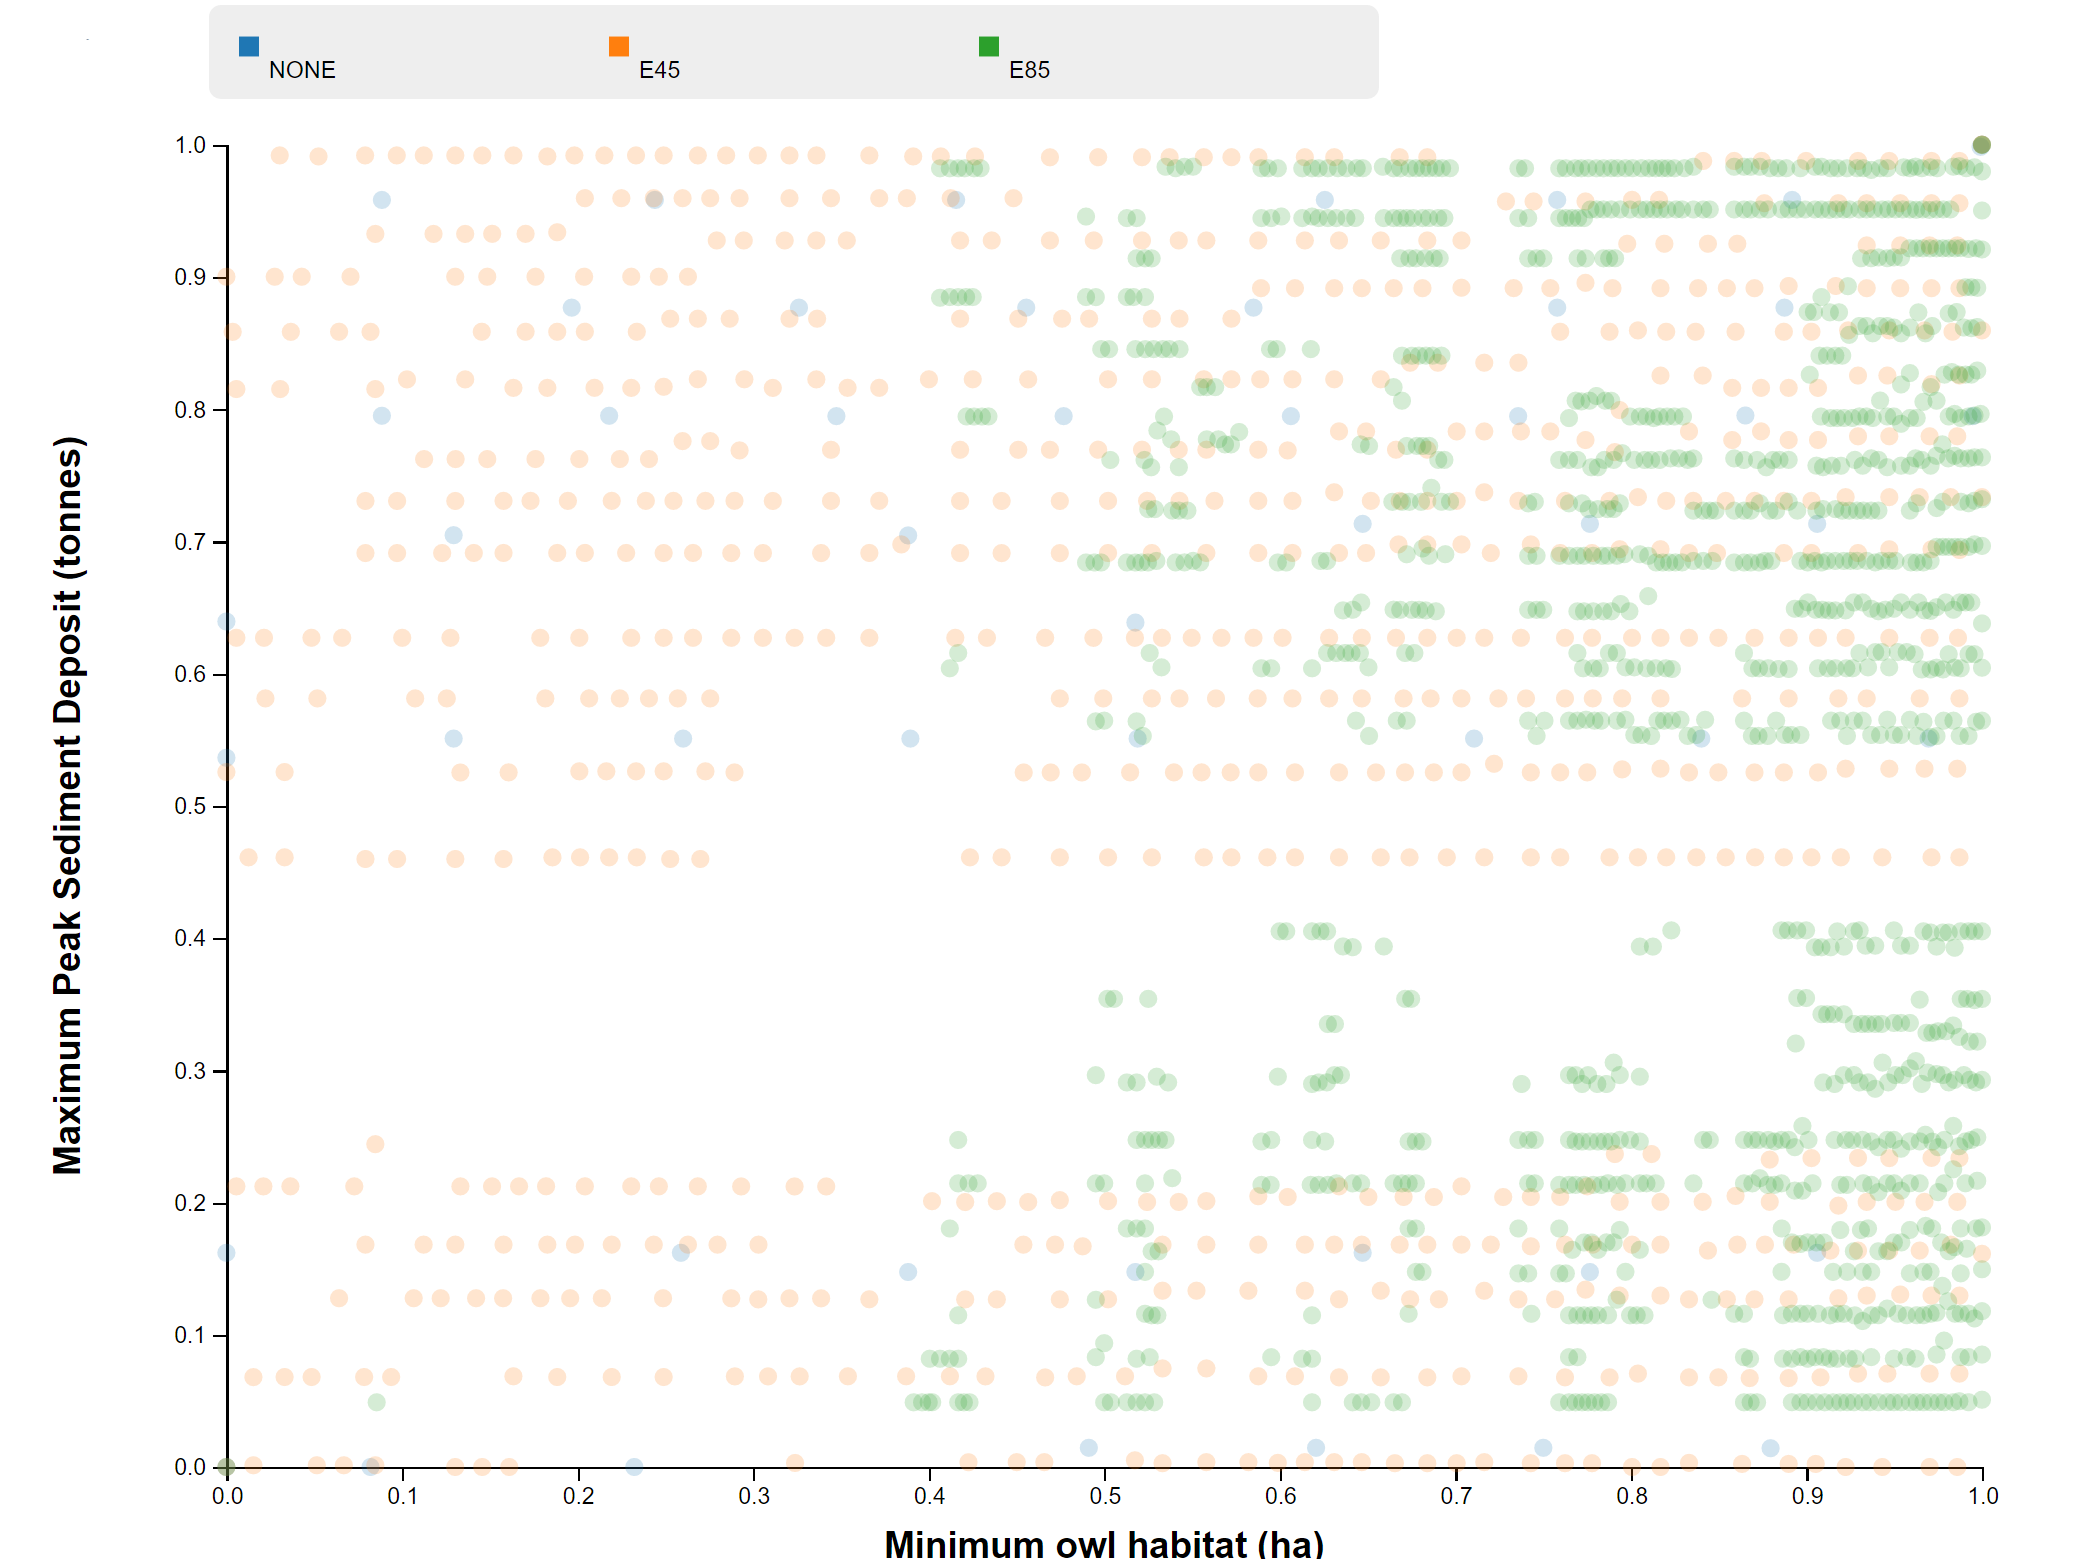
\includegraphics[width=.75\textwidth]{../images/2DSlice_NSO_Sed}
\caption[NSO habitat vs. sediment delivery for all climate scenarios]{NSO habitat versus sediment delivery for all climate scenarios. No obvious conflict pattern exists between the objectives in any climate scenario.}
\label{fig:pairplotNSOSed}
\end{figure}

\paragraph{NSO habitat-fire hazard}
According to $C_{ij}$, the conflict between NSO habitat and fire hazard is again small for all climate scenarios; however, it appears to decrease with increasing severity of climate change. We see in Table \ref{tab:pairConflict-NSOFire} that the average distance to the ideal decreases with increasing severity of climate change. See also Figure \ref{fig:pairplotNSOFire} which shows spreads of solutions for each climate scenario in the NSO habitat-fire hazard plane. The solutions are increasingly more clustered near the sub-dimensional ideal solution with increasing climate change severity.

\begin{figure}[ht]
\centering
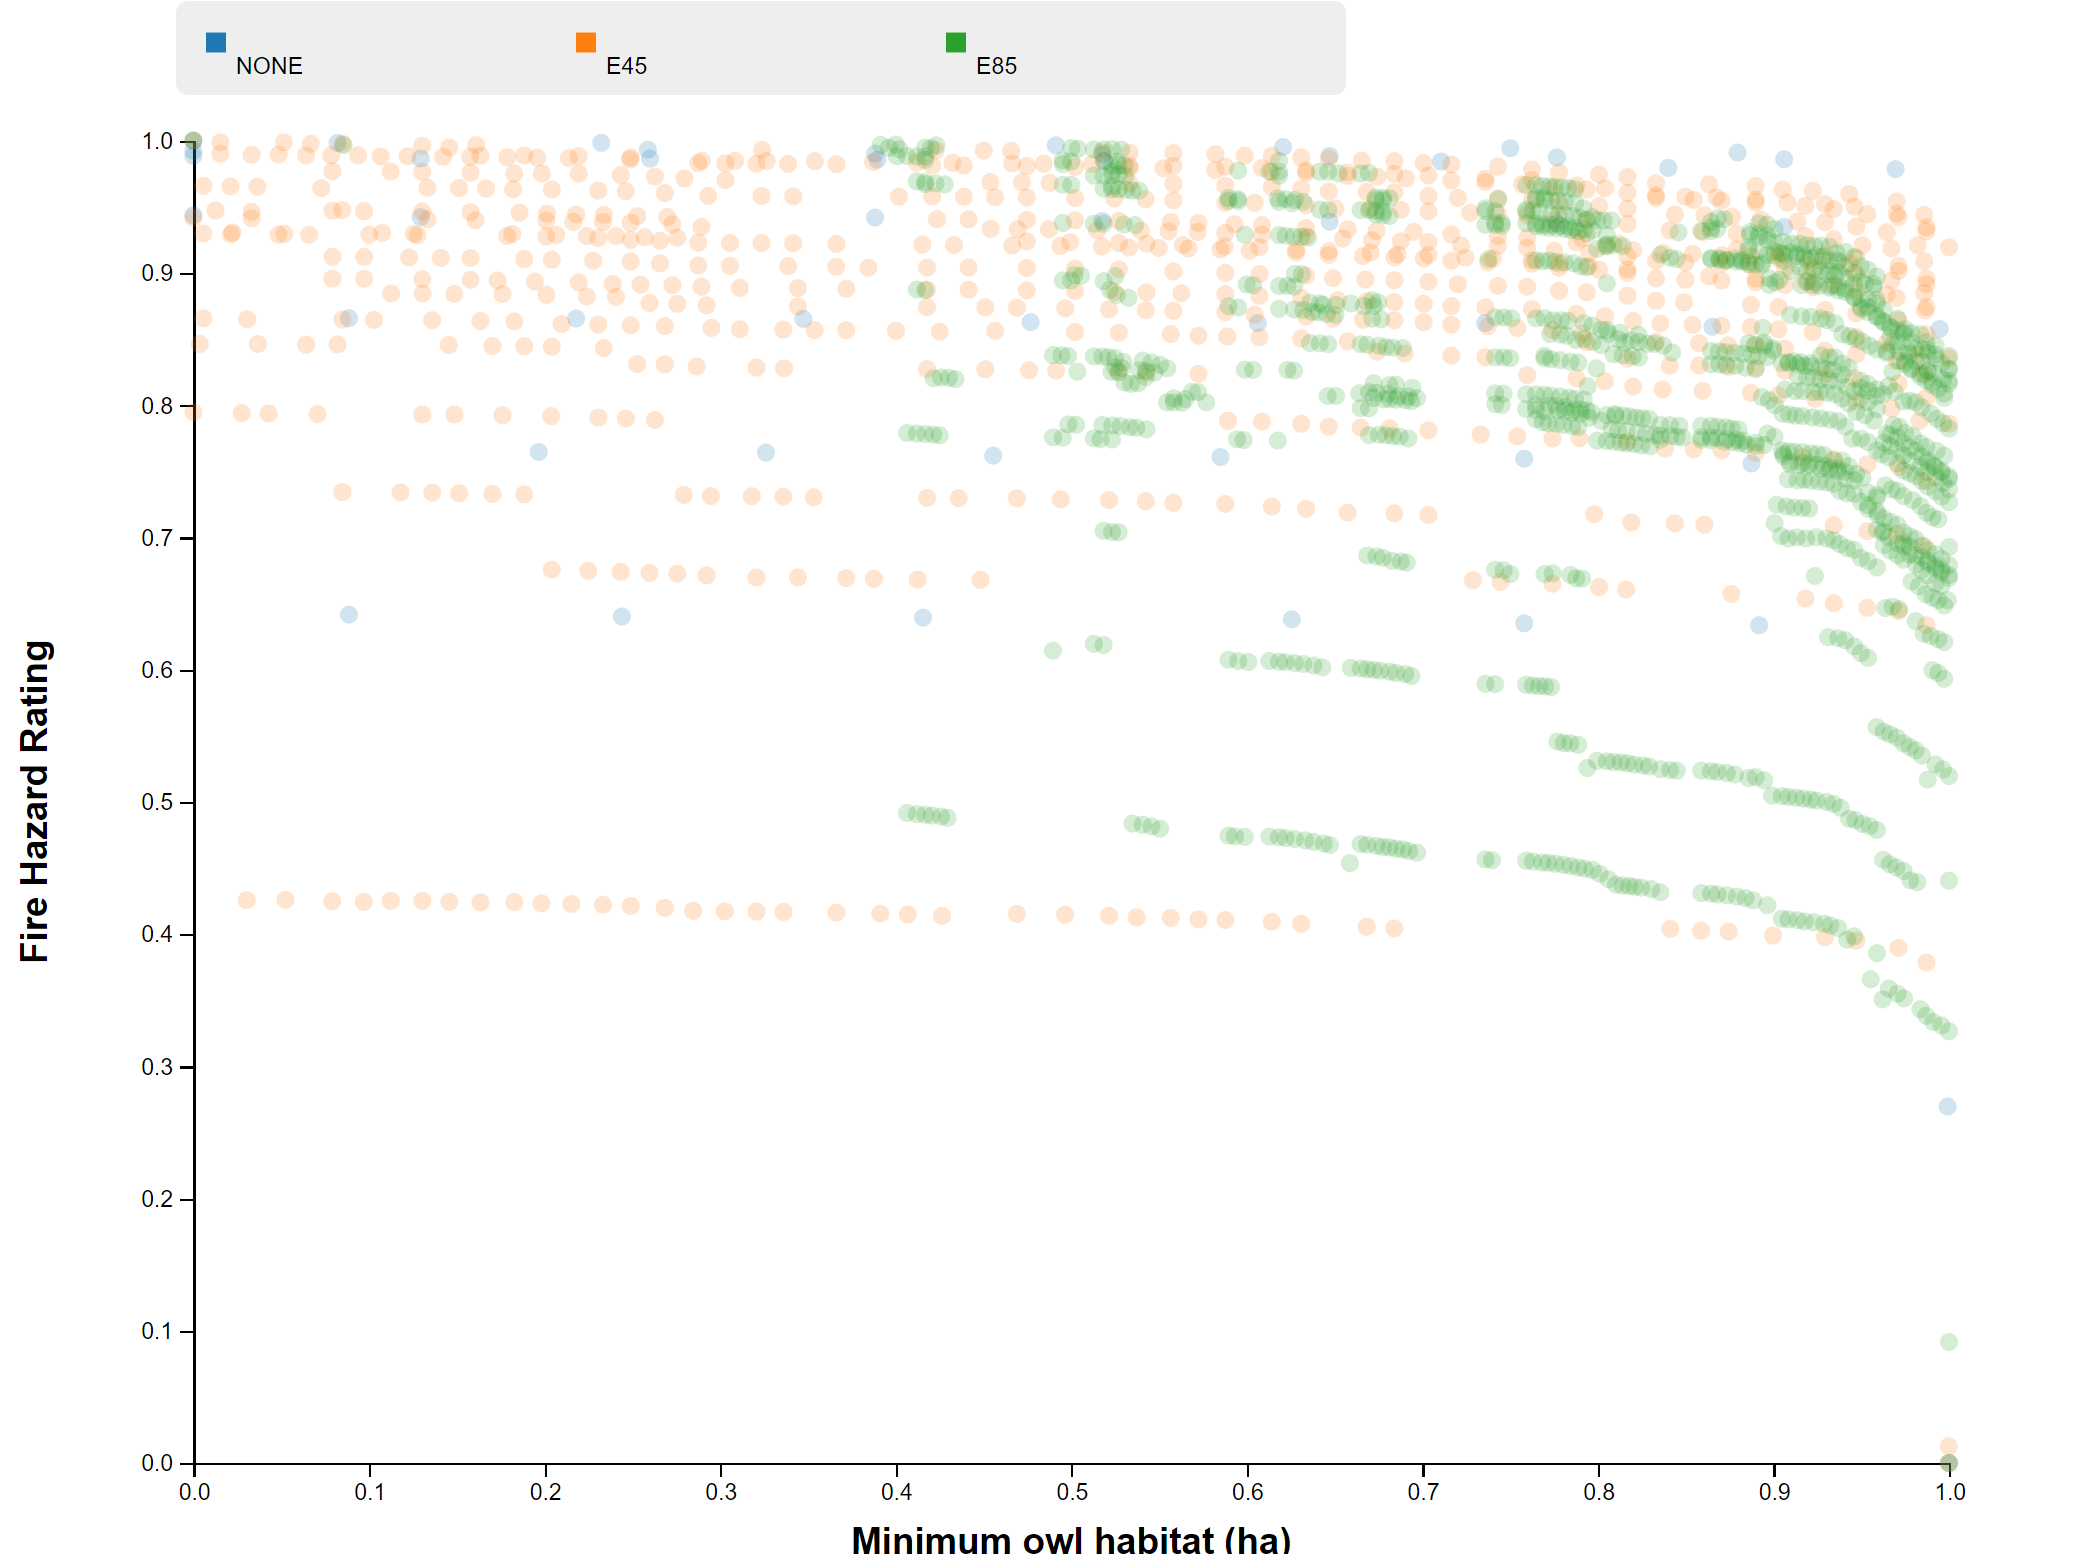
\includegraphics[width=.75\textwidth]{../images/2DSlice_NSO_Fire}
\caption[NSO habitat vs. fire hazard for all climate scenarios]{NSO habitat versus fire hazard for all climate scenarios.}
\label{fig:pairplotNSOFire}
\end{figure}

\begin{table}[]
\centering
\caption[NSO-fire hazard conflict across climate scenarios]{Conflict between NSO habitat and fire hazard across climate scenarios.}
\label{tab:pairConflict-NSOFire}
\begin{tabular}{llll}
\textbf{}     & \textbf{$C_{ij}$} & \textbf{$c_{ij,\rho}$} & \textbf{$c_{ij,d}$} \\ \hline
\textbf{None} & 0.25805           & 0.6622                 & 0.3897              \\
\textbf{E45}  & 0.20560           & 0.5807                 & 0.3541              \\
\textbf{E85}  & 0.15670           & 0.6643                 & 0.2359
\end{tabular}
\end{table}

\paragraph{Fire hazard-sediment delivery}
In all climate scenarios, the strongest pairwise conflict is between fire hazard and sediment delivery. This is apparent from both Figure \ref{fig:pairplotSedFire} and the conflict metric, Table \ref{tab:pairConflict-SedFire}. All rank correlation conflict values $c_{ij,\rho} > 0.95$, indicating strong negative rank correlation. In Figure \ref{fig:pairplotSedFire} we observe a clear void of solutions in all climate change scenarios near the sub-dimensional ideal solution at $(1,1)$; this is unlike Figures \ref{fig:pairplotNSOSed} and \ref{fig:pairplotNSOFire}. We also notice that the None and E45 solutions generally extend beyond the E85 solutions in this plane, seen most clearly near the top-center region of Figure \ref{fig:pairplotSedFire}.

\begin{figure}[ht]
\centering
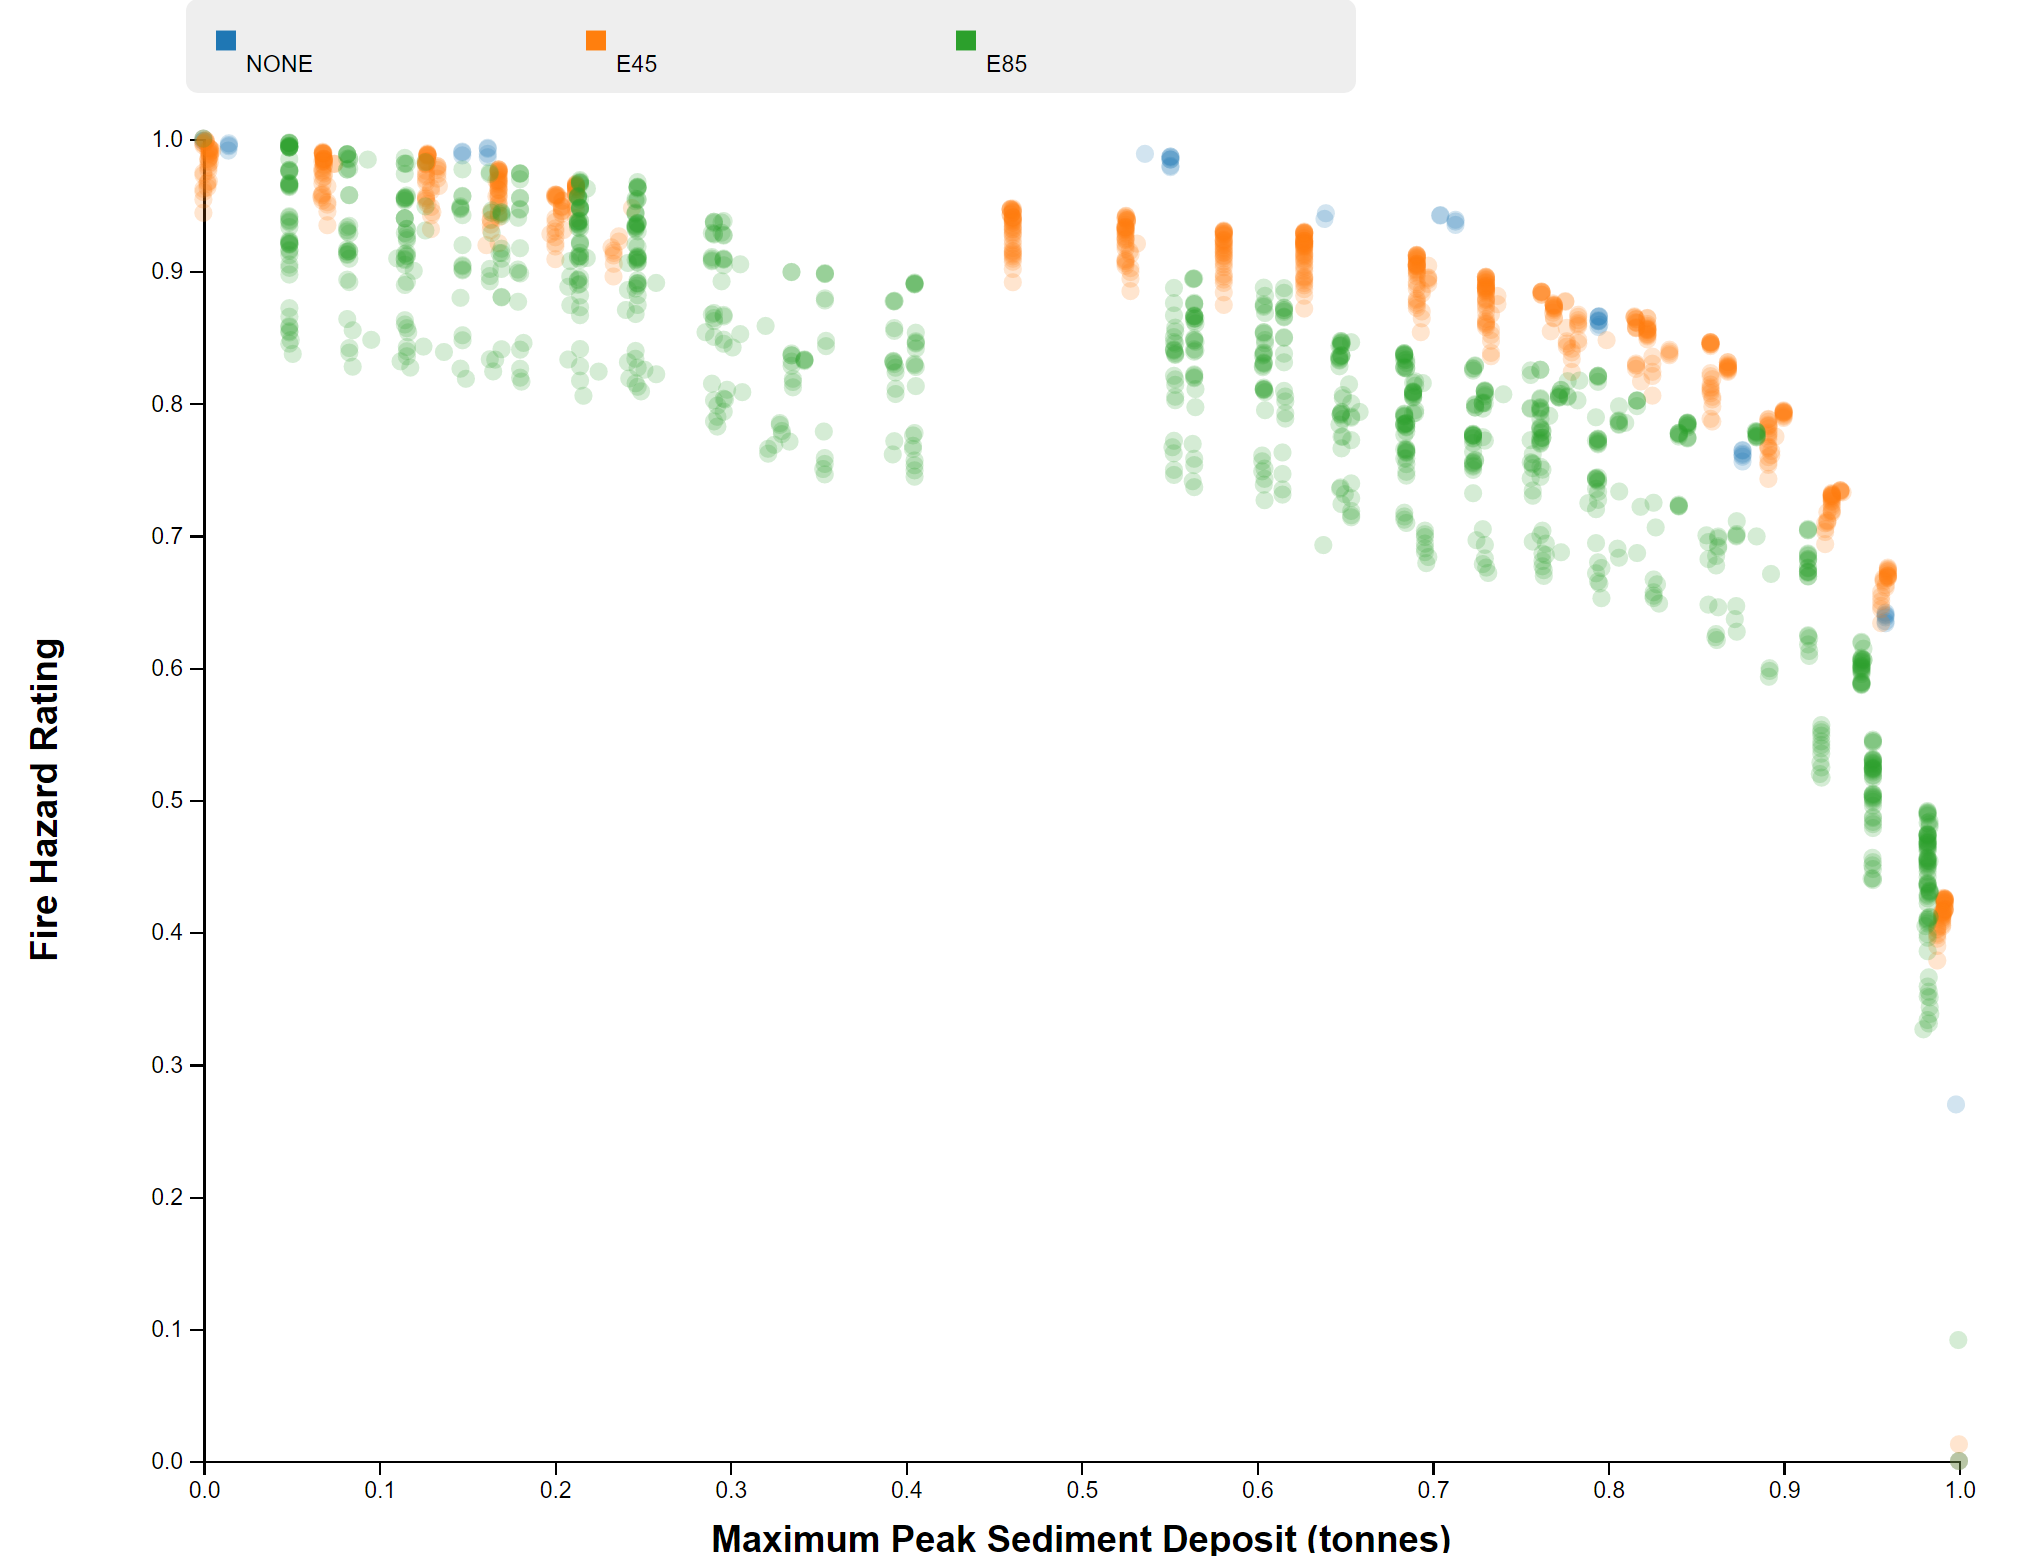
\includegraphics[width=.75\textwidth]{../images/2DSlice_Sed_Fire}
\caption[Sediment delivery vs. fire hazard for all climate scenarios]{Sediment delivery versus fire hazard for all climate scenarios.}
\label{fig:pairplotSedFire}
\end{figure}

\begin{table}[]
\centering
\caption[Sediment delivery-fire hazard conflict across climate scenarios]{Conflict between sediment delivery and fire hazard across climate scenarios.}
\label{tab:pairConflict-SedFire}
\begin{tabular}{llll}
\textbf{}     & \textbf{$C_{ij}$} & \textbf{$c_{ij,\rho}$} & \textbf{$c_{ij,d}$} \\ \hline
\textbf{None} & 0.36039           & 0.9927                 & 0.3630              \\
\textbf{E45}  & 0.36097           & 0.9853                 & 0.3664              \\
\textbf{E85}  & 0.38261           & 0.9514                 & 0.4021
\end{tabular}
\end{table}

\section{Discussion}
We divide our discussion of results into three sections: first, the decreasing provision of individual ecosystem services with climate change; second, the increase in the number of solutions and in the range of NSO habitat available; and third, conflict and the joint provision of ecosystem services.


\subsection{Conflict and the joint provision of ecosystem services}
We observe a decreasing hypervolume with increasing climate change severity. Lower values for the hypervolume are indicative of more conflict, meaning that climate change induces more conflict among the ecosystem services and leads to less joint provision of objectives.

The difference in hypervolume between None and E45 $I_{H1}(Z_\text{None}) - I_{H1}(Z_\text{E45}) \approx 0.01$. Recall that a difference of $h$ in hypervolumes equates to a difference of $h^{1/M}$ in each objective (Figure \ref{fig:Hypervol10percent}). Thus, despite the small size of the difference between $I_{H1}(Z_\text{None})$ and $I_{H1}(Z_\text{E45})$, it signifies an additional joint provision of objectives of approximately 21.6\%. This difference is greater between None and E85, approximately 0.05, representing an additional joint provision of ecosystem services of approximately 36.2\%.

From the hypervolumes alone, it is uncertain whether None represents a strictly better frontier than either E45 or E85 or if, despite their smaller hypervolume values, E45 and E85 enclose some region of the objective space that is not enclosed by None. Any such region would extend further into the objective space, representing the presence of solutions that achieve greater joint provision of ecosystem services. The results of the binary hypervolume were presented in Table \ref{tab:binaryHypervols}.

The results show that no frontier is dominated by any other, and each frontier encloses some region of the objective space not enclosed by the others. For the pairs of frontiers for which the binary hypervolume is greatest ($(Z_\text{None},Z_\text{E85})$ and $(Z_\text{E45},Z_\text{E85})$), this additional extension into the objective space is most obvious in Figure \ref{fig:pairplotSedFire}. We see for values of sediment delivery between 0.15 and 0.8 that None appears to dominate E45 which appears to dominate E85. Further, for sediment delivery values between 0.8 and 1, it appears that E45 dominates E85 and None, between which any domination relationship is difficult to discern.

The existence of these areas leads to the lower value of conflict $C_{ij}$ between sediment delivery and fire hazard in None and E45 than in E85. We note the success of the conflict metric $C_{ij}$ here: all frontiers in the sediment delivery-fire hazard plane of Figure \ref{fig:pairplotSedFire} are similar. They have similar shape and achievement towards the sub-dimensional ideal solution, yet the metric is able to distinguish differences in conflict between them.

For the other pairwise objective comparisons, as we saw in Figures \ref{fig:pairplotNSOSed} and \ref{fig:pairplotNSOFire}, the distribution of solutions more closely resembles a uniform two-dimensional scattering. There is no clear conflict pattern between them like that which we saw in Figure \ref{fig:pairplotSedFire}. As a result, $C_{ij}$ reports little conflict between these objective pairs, as desired. However it varied in unexpected ways between the climate scenarios. In these cases, we find that the distance component $c_{ij,d}$ was primarily responsible for the variations, as the rank correlations tended to be insignificantly different from 0.5. It appears the conflict metric $C_{ij}$ is susceptible to such variations when neither the $c_{ij,d}$ nor $c_{ij,\rho}$ component tends towards their limiting values of 0 and 1.

% In general, however, it was really awesome.
However, in general, we find our process of utilizing the hypervolume measures and the proposed conflict metric to have been successful in quantifying conflict within and among the frontiers. The pairwise conflict metric successfully identified the pair of objectives which demonstrated the most conflict, and the hypervolumes indicated which climate scenarios allow for greater joint provision of ecosystem services.